\documentclass[tikz]{standalone}
\usepackage{pgfplots}
\pgfplotsset{compat=1.15}
\usepackage{mathrsfs}
\usetikzlibrary{arrows,calc}
\usepackage{tkz-euclide}

\pagestyle{empty}

\definecolor{AngleClr}{rgb}{0,0.39215686274509803,0}
\definecolor{ShapeClr}{rgb}{0.6,0.2,0}

\begin{document}

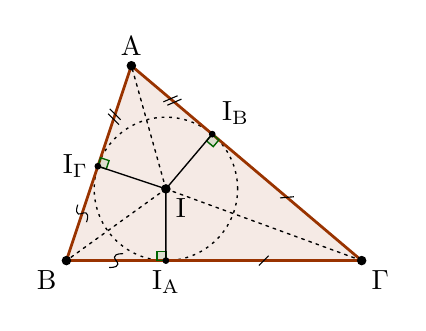
\begin{tikzpicture}[scale=.75]
\tkzSetUpLine[line width=1pt,color=black]
\tkzSetUpPoint[fill=black]

\tkzDefPoints{0/0/B,1.1/3.3/A,5/0/C}

\tkzDefTriangleCenter[in](A,B,C) \tkzGetPoint{I}

\tkzDefPointBy[projection=onto B--C](I)\tkzGetPoint{IA}
\tkzDefPointBy[projection=onto A--C](I)\tkzGetPoint{IB}
\tkzDefPointBy[projection=onto A--B](I)\tkzGetPoint{IC}

\tkzInterLL(A,IA)(B,IB) \tkzGetPoint{GE}

\tkzFillPolygon[fill=ShapeClr,fill opacity=0.1](A,B,C)

\tkzDrawCircle[line width=0.5pt,color=black,dashed,dash pattern=on 1pt off 1.75pt](I,IA)

\tkzDrawPolygon[color=ShapeClr](A,B,C)


\tkzMarkRightAngles[line width=0.5pt, size=.15,color=AngleClr,fill=AngleClr,fill opacity=0.1](I,IA,B I,IB,C I,IC,A)

\tkzDrawSegments[line width=0.5pt,color=black,dashed,dash pattern=on 1pt off 1.75pt](I,A I,B I,C)
\tkzDrawSegments[line width=0.5pt,color=black](I,IA I,IB I,IC)

\tkzDrawPoints[size=3](A,B,C,I)
\tkzDrawPoints[size=2](IA,IB,IC)
\tkzLabelPoint[above](A){$\rm A$}
\tkzLabelPoint[below left](B){$\rm B$}
\tkzLabelPoint[below right](C){$\rm \Gamma$}
\tkzLabelPoint[below](IA){$\rm I_A$}
\tkzLabelPoint[above right](IB){$\rm I_B$}
\tkzLabelPoint[left](IC){$\rm I_\Gamma$}
\tkzLabelPoint[below right](I){$\rm I$}

\tkzMarkSegments[mark=s|,size=2.5](IA,C IB,C)
\tkzMarkSegments[mark=s||,size=2.5](A,IB A,IC)
\tkzMarkSegments[mark=s,size=2.5](B,IA B,IC)

\end{tikzpicture}

\end{document}
